\documentclass[a4paper,12pt,leqno,titlepage]{article}
\usepackage{hyperref} %linkitys
\usepackage{graphicx}
\usepackage{listings}
\usepackage{moreverb}
\usepackage{amsmath}
\usepackage{amsthm}
\usepackage[english]{babel}
%\usepackage[finnish]{babel}
\usepackage{ucs}
\usepackage[utf8x]{inputenc}
\usepackage{amssymb}
\newcommand{\R}{\mathbb{R}} %lukujoukkosymbolit
\newcommand{\C}{\mathbb{C}}
\newcommand{\Q}{\mathbb{Q}}
\newcommand{\N}{\mathbb{N}}
\newcommand{\Z}{\mathbb{Z}}
\newcommand{\logM}{\mathcal{M}}
\newcommand{\bigO}{\mathcal{O}}
\setlength{\parindent}{0pt} %kappalejakoa
\setlength{\parskip}{2ex}
\newcommand{\compcent}[1]{\vcenter{\hbox{$#1\circ$}}}
\newcommand{\comp}{\mathbin{\mathchoice
{\compcent\scriptstyle}{\compcent\scriptstyle}
{\compcent\scriptscriptstyle}{\compcent\scriptscriptstyle}}}

%\hyphenpenalty=750
%\setlength{\emergencystretch}{1.5 em} % Tavutusasetukset suomen kielelle

\hypersetup{
pdfborder = {0 0 0 0}, %linkkien värejä etc kikkailua
colorlinks = true,
linkcolor = black,
urlcolor = blue,
citecolor = red,
}


\usepackage{lastpage} %sivumäärä alaviitteeseen
\usepackage{fancyhdr}

\pagestyle{fancy}
\cfoot{Page \thepage/\pageref{LastPage}} % \\ Opiskelijanumero 013126382}


\begin{document}
\begin{titlepage}
\title{Data structures project, \\
Testing document}
\author{Heikki Haapala and Aleksi Markkanen\\
Student numbers 014090190 and 013126382\\
\pageref{LastPage} pages}
\date{\today}
\end{titlepage}
\maketitle
\pagebreak
\tableofcontents
\pagebreak



\begin{comment}
Testausdokumentti
Mitä on testattu, miten tämä tehtiin
Minkälaisilla syötteillä testaus tehtiin (vertailupainotteisissa töissä tärkätä)
Miten testit voidaan toistaa
Ohjelman toiminnan empiirisen testauksen tulosten esittäminen graafisessa muodossa.
\end{comment}

\section{Introduction}
The program was tested using \emph{JUnit} tests during developement.
The tests include cases for degenerate hulls and also contain normally distributed 2D point sets.

The correct output was verified using \emph{Octave}, and correct results were saved so that the \emph{JUnit} tests could check the output of the program.


\pagebreak
\section{Inputs Used in Tests}
Different distributions were used as inputs during testing; these include normal distribution, exponential distribution and uniform distribution. We also used a combination of different distributions for x and y coordinates, respectively.

Testing was conducted with and without the \emph{Akl-Toussaint heuristic}.

We also implemented a simple iteration functionality to the program and this allowed us to capture average running times.
This eliminates interferance from other running processes.


\pagebreak
\section{Running the Tests}

\pagebreak
%\section{Ohjelman toiminnan empiirisen testauksen tulosten esittäminen graafisessa muodossa}
\section{Graphical Presentation of the Results of the Empirical Testing of the Correctness of the Program}
\begin{figure}[h!]
\caption{A picture of a gull.} %convex hull}
\centering
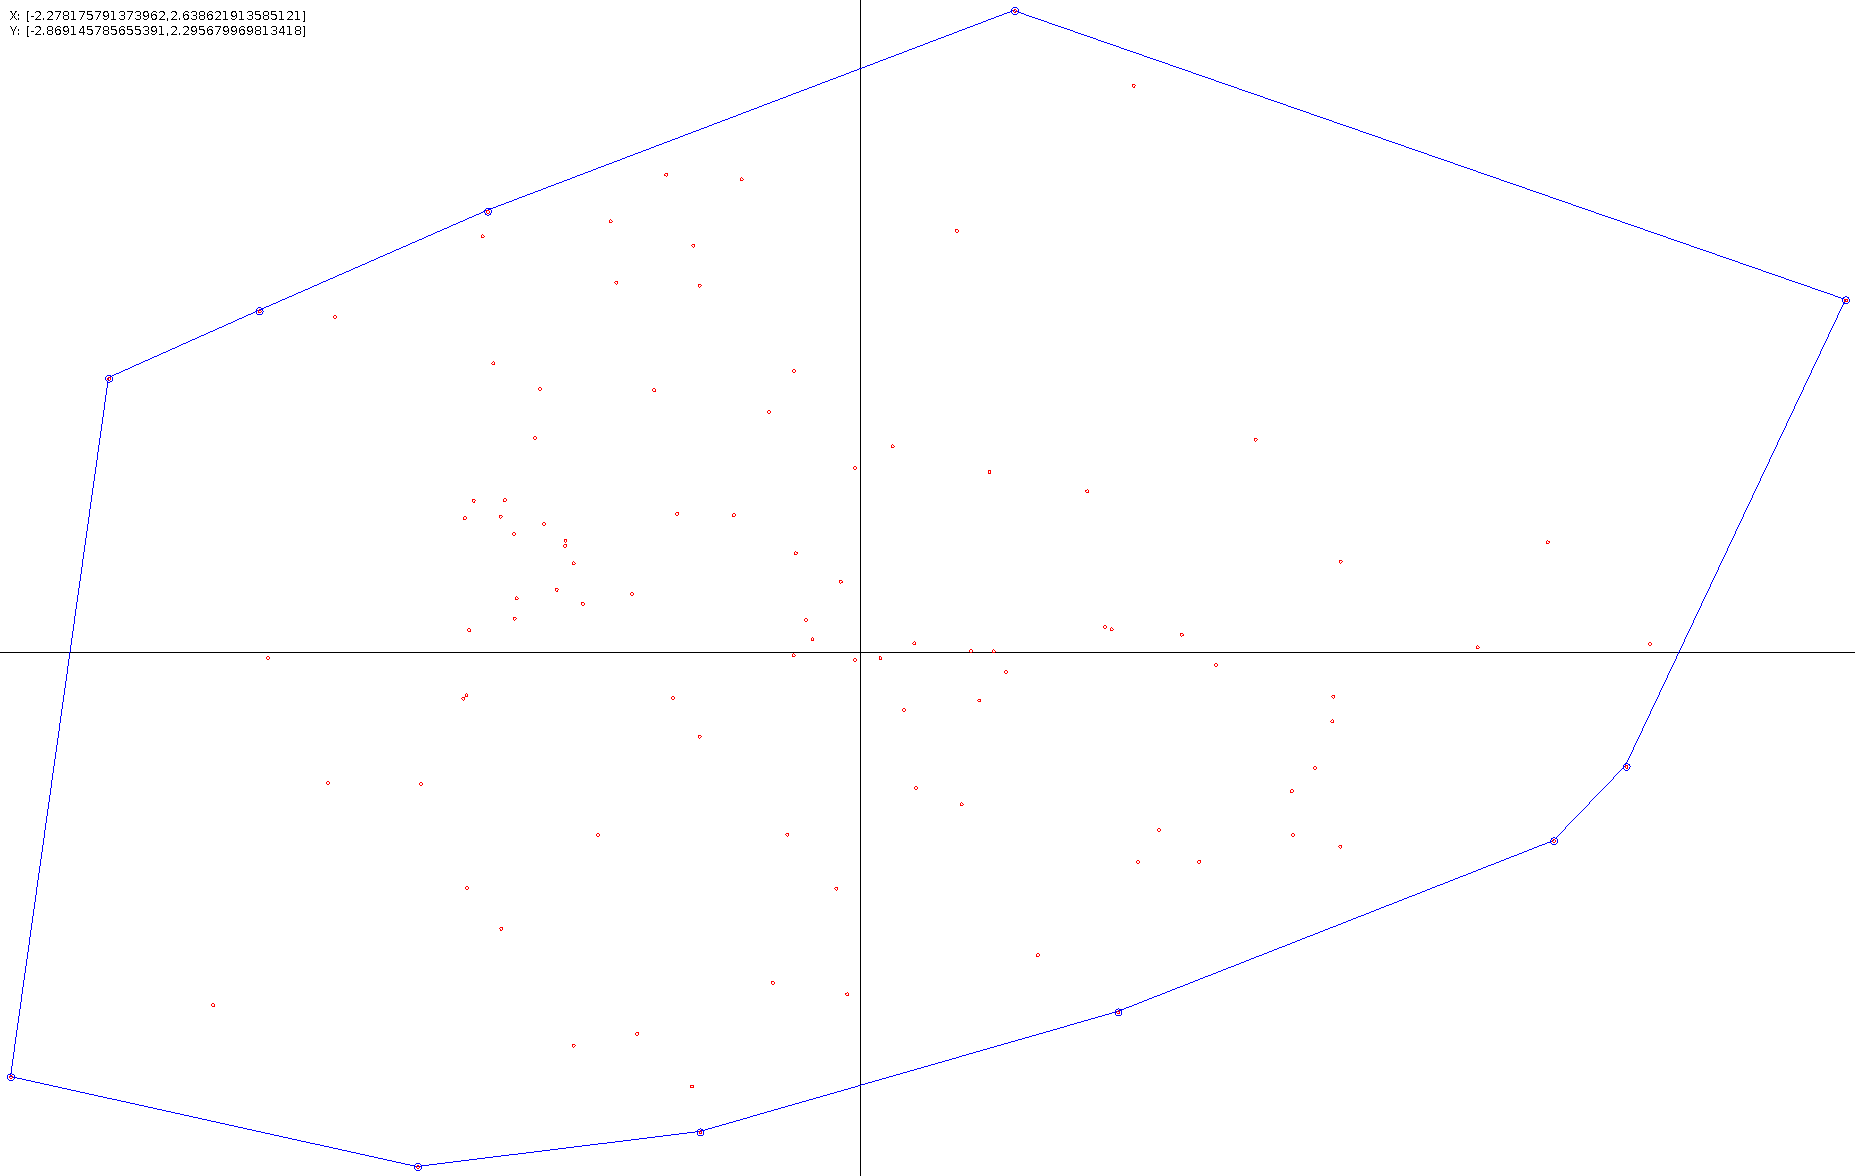
\includegraphics[width=\textwidth]{gull.png}
\end{figure}

\pagebreak


\begin{thebibliography}{9}
\bibitem{wiki}

Convex hull algorithms,

Wikipedia, the free encyclopedia

\url{http://en.wikipedia.org/wiki/Convex_hull_algorithms}


\end{thebibliography}

\end{document}
